\documentclass[10pt, twocolumn]{jarticle}
\usepackage[caption=false]{subfig}
\usepackage{amsmath}
\usepackage{amsfonts}
\usepackage{algorithmic}
\usepackage{algorithm}
\usepackage[dvipdfmx]{graphicx}
\usepackage{bm}
\usepackage{setspace}
\usepackage{url}
\usepackage[tiny]{titlesec}

\renewcommand{\figurename}{\small 図}
\renewcommand{\tablename}{\small 表}

% 余白の上を25mm、下を20mmに
\setlength{\textheight}{\paperheight}
\addtolength{\textheight}{-45truemm}
\setlength{\topmargin}{-0.4truemm}
\addtolength{\topmargin}{-\headheight}
\addtolength{\topmargin}{-\headsep}

% 余白の左を20mm、右を20mmに
\setlength{\textwidth}{\paperwidth}
\addtolength{\textwidth}{-40truemm}
\setlength{\oddsidemargin}{-5.4truemm}

% ヘッダの設定
\usepackage{fancyhdr}
\pagestyle{fancy}
\rhead{}
\lhead{\bf 2019年度 工学部システム創成学科PSI コース 卒業論文概要}
\renewcommand{\headrulewidth}{0pt}

% 2つのカラムの間隔を設定
\setlength{\columnsep}{8mm}

% 題目の設定
\titleformat{\section}{\bf \fontsize{10pt}{12pt}}{\thesection.}{1zw}{}
\titleformat{\subsection}{\bf \fontsize{10pt}{12pt}}{\thesubsection.}{1zw}{}
\titlespacing{\section}{0pt}{*3}{*0}
\titlespacing{\subsection}{0pt}{*3}{*0}

%%%%%%%%%%%%%%%%%%%%%%%%%%%%%%%%%%%%%%%%%%%%%%%%%%
\begin{document}

\twocolumn[%
\begin{center}
{\bf \fontsize{14pt}{16pt}\selectfont 複雑環境下でのロボット学習に向けた\\深層状態空間モデルを用いた映像予測}  % 論文題目
\end{center}
\begin{flushright}
\fontsize{11pt}{13pt}\selectfont 03-180961 近藤生也\\% 学籍番号、氏名
\fontsize{11pt}{13pt}\selectfont 指導教員 松尾豊 教授% 指導教員名
\end{flushright}
]%

% 行間を0.8倍に
\setstretch{0.8}

%%%%%%%%%%%%%%%%%%%%%%%%%%%%%%%%%%%%%%%%%%%%%%%%%%
% 以下、本文
\section{序論}

近年,機械学習・深層学習を用いてロボットの制御方法をロボット自らに学ばせる{\bf ロボット学習}の研究が進んでおり,ロボットの実用化の可能性が広がっている.ロボット学習において{\bf 映像予測}は重要であり,ロボット自身の行動計画の作成や\cite{hafner2019planet},ユーザーが事前にロボットの行動を評価する際に用いることができる\cite{ebert2018visual}.映像予測のアプローチは大きく{\bf 回帰型ニューラルネットワーク}ベースの手法と{\bf 深層状態空間モデル}ベースの手法に分けられる.前者は生成精度は高いが長期の予測の際には誤差が蓄積しやすく,また予測を行うには直前までの映像を複数フレーム用意する必要があり予測してから行動したいようなロボット実機の問題設定には向いていない.一方後者は近年深層強化学習の分野で用いられており,ゲームや単純なシミュレーターを題材にした映像予測は可能なものの,複雑なデータに対してはRNNベースの手法と比較し高精度な予測が難しく,映像予測自体を目的にした研究は進んでいない.

本研究ではロボット学習への応用を前提とし,DSSMをベースにした映像予測性能の向上を目指す.提案手法として,状態表現の階層性に着目したDSSMの拡張を考え,実験によりその有効性を示す.

\section{前提知識}
\subsection{DSSM}
{\bf 深層状態空間モデル(Deep State Space Model,DSSM)}は将来の観測の予測を通して環境の状態表現を獲得する深層学習手法である\cite{krishnan2015deep}.DSSMのグラフィカルモデルは図\ref{fig:ssm}のように表され,各時刻の状態表現$s_t$の遷移とその時刻の観測$o_t$の生成過程をニューラルネットワークで表現する.DSSMは初期状態$s_0$と環境中の行動主体の行動系列$a_{1:T}$を入力とし,$o_{1:T}$を予測し出力することができる.ただし初期状態は$o_0$から求められる.

\begin{figure}[h]
  \begin{center}
    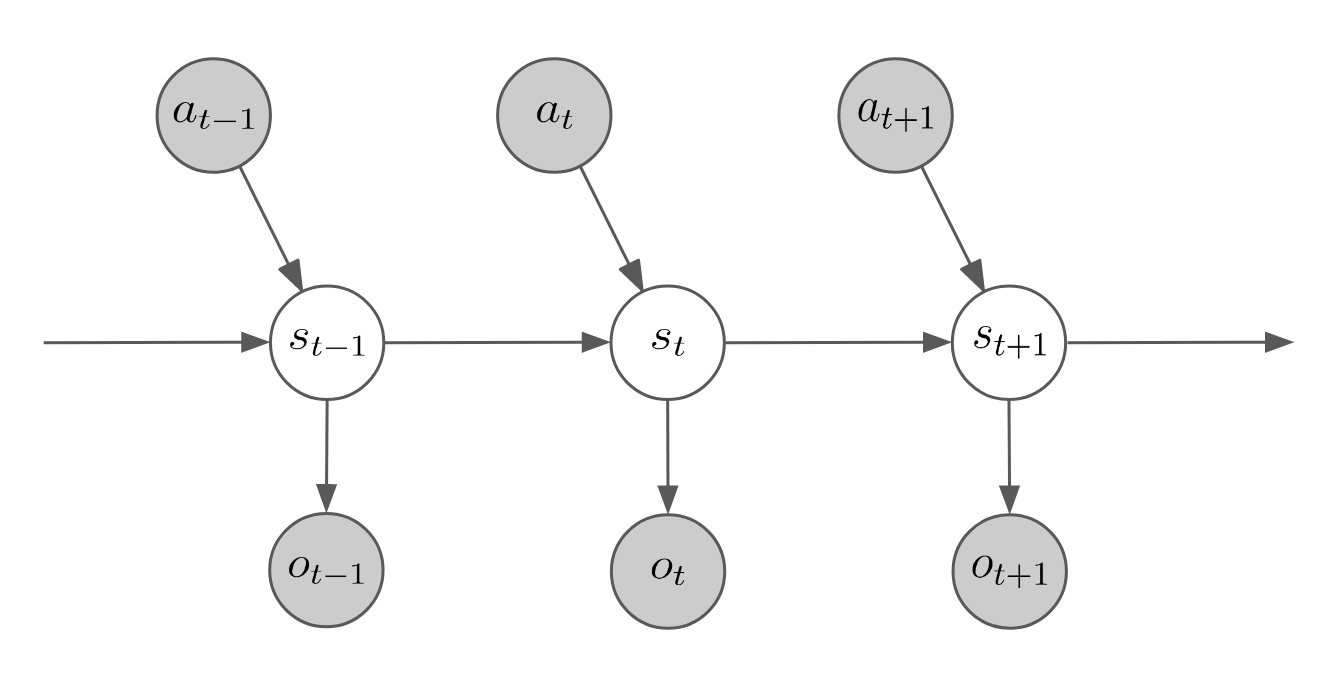
\includegraphics[width=0.8\linewidth]{./figures/dssm.png}
    \caption[DSSMのグラフィカルモデル]{\small DSSMのグラフィカルモデル.実線は生成分布,点線は推論分布を表す.簡単のため推論分布は時刻tでのみ記載している.}
    \label{fig:ssm}
  \end{center}
\end{figure}

DSSMのネットワークのパラメータは,図\ref{fig:ssm}の点線で表された推論分布$q(s_t|s_{t-1}, a_t, o_t)$を導入することで,次の変分下限の最大化によって求められる.
\small
\begin{eqnarray}
  \log p(o_{1:T}|a_{1:T}) \geq \sum_{t=1}^T ( {L}_{reconst} - {L}_{KL}) 
\end{eqnarray}
ただし,
\begin{eqnarray}
  && {L}_{reconst} = \mathbb{E}_{s_t \sim q(s_t|s_{t-1}, a_t, o_t)} [\log p(o_t|s_t)] \nonumber \\
  && {L}_{KL} = \mathbb{E}_{s_{t-1} \sim q(s_{t-1}|s_{t-2}, a_{t-1}, o_{t-1})} \nonumber \\
  && \hspace{2em} [\mathrm{D_{KL}}(q(s_t|s_{t-1}, a_t, o_t) \| p(s_t|s_{t-1}, a_t, o_t, s_t))] \hspace{6em} \nonumber
  \label{eq:dssm_elbo}  
\end{eqnarray}
\normalsize
ここで$ - L_{reconst}$は観測の再構成誤差を,$L_{KL}$は$s_t$の生成分布と近似分布の間のカルバック・ライブラー情報量を指す.

\section{問題設定}
本研究では{\bf 行動条件付き映像予測}の問題を扱う.具体的には,行動系列と観測系列の組$\{\vec{a},\vec{o}\}$の訓練用のデータを用いて学習し,評価用のデータで初期観測$o_0$と行動系列$a_{1:10}$が与えられたときに正しく$o_{1:10}$の予測・生成ができることを目指す.本研究ではBAIR Push Dataset\cite{ebert2017selfsupervised}を用いて各手法の評価を行う.

\section{深層状態空間モデルの問題点}
予備実験としてDSSMを用いてBAIR Push Datasetで学習を行った際の学習曲線を図\ref{fig:curve}のBaseline(64) $\sim$ (1024)に示す.ただし括弧内の数字は状態変数$s_t$の次元数である.モデルが状態表現として獲得できる情報量を増やすためには素朴には状態変数の次元を大きくすることが考えるが,実際には学習がうまく進まず,性能はむしろ下がることがわかった.これを受けて潜在変数の次元を大きくした際にも学習をうまく進める方法を考える.

% \caption[hoge]{fuga}
\begin{figure}[h]
  \begin{center}
    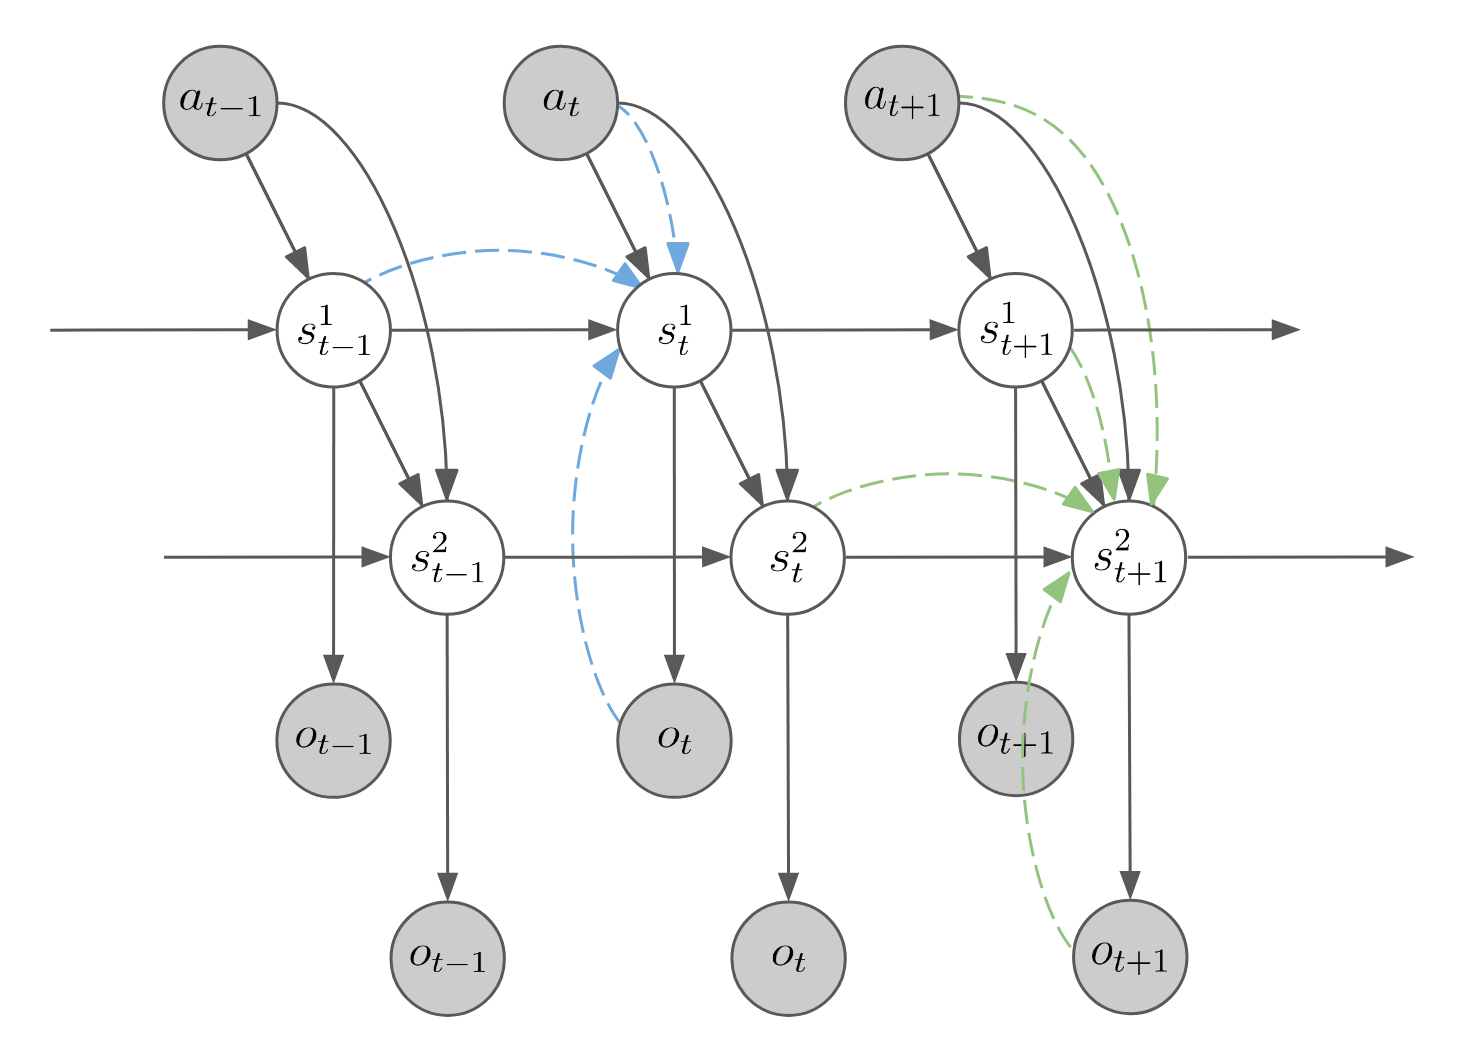
\includegraphics[width=\linewidth]{./figures/proposal_train.png}
    \caption[提案手法(二階層)のグラフィカルモデル]{\small 提案手法のグラフィカルモデル.実線が生成分布,点線が推論分布を示す.また2つずつ記載されている$o_t$は同じデータを示すが.異なるsから独立に生成されることを明示している.}
    \label{fig:proposal}
  \end{center}
\end{figure}

\begin{algorithm}[h]               
  \caption{\small N階層DSSMの学習アルゴリズム}
  \label{alg1}
  \begin{algorithmic}
    \REQUIRE \small 階層数 $N$ 
    \FOR{i = 1 to $N$}
      \WHILE{\small $i$ 階層の学習が収束していない}
        \STATE \small $1 \sim i-1$階層のパラメータを固定し, 
        \STATE \small $i$階層を次の目的関数$L$で学習する
        \STATE $\hspace{1em} L(a_{1:T}, o_{1:T}) = \sum_{t=1}^T ( {L^i}_{reconst} - {L^i}_{KL}) $
        \STATE where, 
        \STATE $\hspace{1em} {L^i}_{reconst} = \mathbb{E}_{s^i_t} [\log p(o_t|s^i_t)]$
        \STATE $\hspace{1em} {L^i}_{KL} = \mathbb{E}_{s^i_{t-1}} [\mathrm{D_{KL}}(q(s^i_t|s^i_{t-1}, a_t, o_t) \| $
        \STATE $\hspace{9em} p(s^i_t|s^i_{t-1}, a_t, o_t, s^{i-1}_t))] )$
      \ENDWHILE
    \ENDFOR
  \end{algorithmic}
\end{algorithm}

\section{状態表現の階層性を考慮することによる\\深層状態空間モデルの拡張}
\label{chap:proposal}
状態変数の次元を大きくすると,状態変数の遷移の部分で高次元変数から高次元変数への変換を学習する必要が生じ全体の学習が困難になる.そこで高次元の状態表現の学習時に小さい状態変数で学習した各時刻の状態表現を補助的に用いることを考え,図\ref{fig:proposal}のグラフィカルモデルで表されるDSSMの拡張を提案する.またこのモデルの学習アルゴリズムをアルゴリズム\ref{alg1}に示す.モデルの評価時には,最高層の状態変数から観測への生成過程 $p(o_t|s^N_t)$ を用いる.

\section{実験}
\label{chap:experiment}

\subsection{実験内容}

提案手法とベースラインの比較実験を行う.提案手法は64次元と512次元の二階層の状態ベクトルを持つモデルと,64次元と512次元と1024次元の三階層の状態ベクトルを持つモデルで実験を行った.

\subsection{実験結果}

\begin{figure}[h]
    \begin{center}
        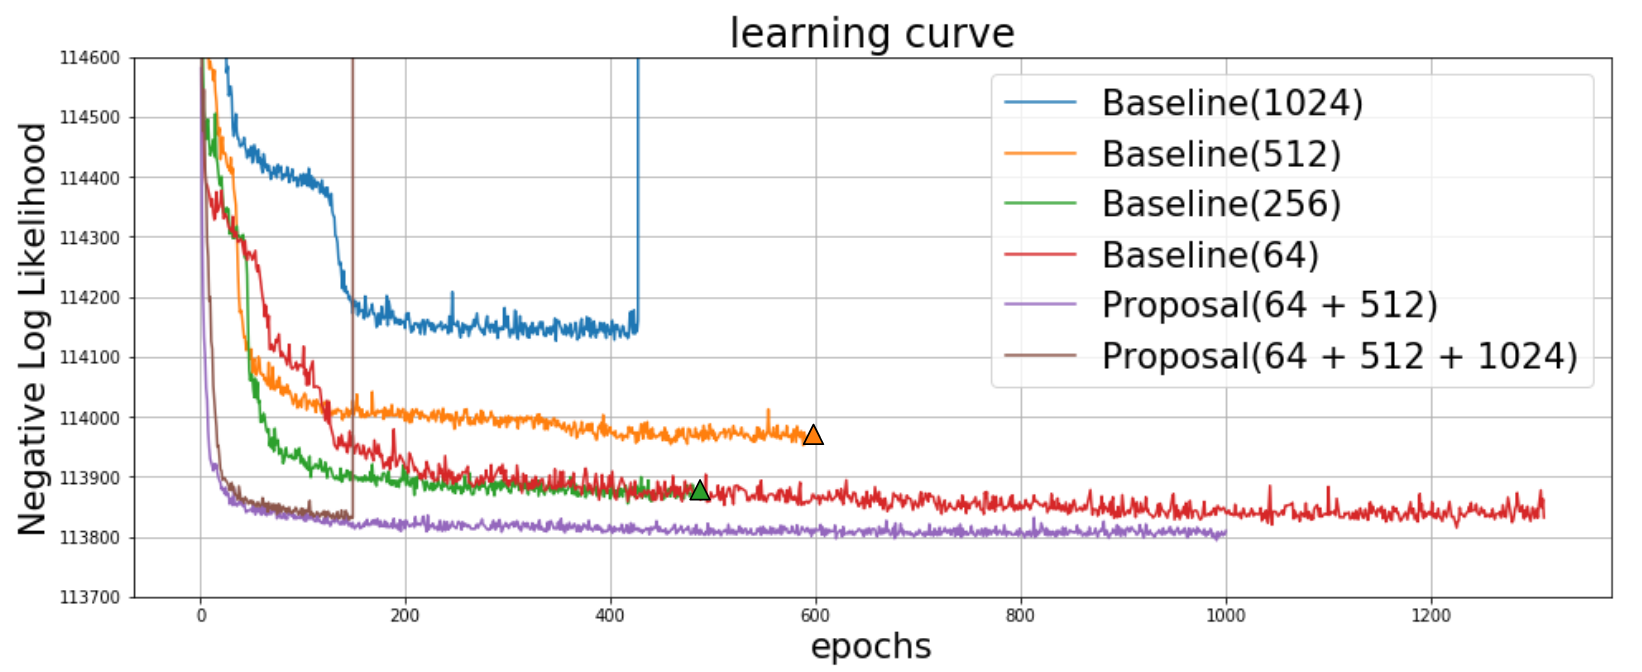
\includegraphics[width=\linewidth]{./figures/curve_yoko.png}
        \caption[提案手法の学習曲線]{\small ベースラインと提案手法の学習曲線.グラフ中に三角で示されるのは目的関数の値にNanが出力されたことを示す.}
        \label{fig:curve}
    \end{center}
    \end{figure}
\normalsize

% \begin{table}[h]
%     \begin{center}
%     \caption{\small 手法ごとの定量評価指標(尤度)}
%     \begin{tabular}{|c||c|} \hline
%       \small 手法 & \small 負の対数尤度 \\ \hline \hline
%       \small ベースライン(64) & \small $1.1384 \times 10^5 $ \\ \hline
%       \small 提案手法(64 + 512) & \small $\bm{1.1381 \times 10^5 }$ \\ \hline
%       \small 提案手法(64 + 512 + 1024) & \small $1.1383 \times 10^5$ \\ \hline
%     \end{tabular}
%     \label{table:evaluation}
%     \end{center}
%   \end{table}
% \normalsize


% 簡単のため,ここから状態変数の次元を64にしたベースラインモデルを「ベースライン(64)」,状態変数の次元を64と512にした提案手法モデルを「提案手法(64 + 512)」などと呼ぶ.


図\ref{fig:curve}に各モデルの学習曲線を示す.ベースラインでは状態変数の次元を512, 1024と大きくすると学習が進まなかったが,提案手法では学習が進みさらに二階層・三階層モデルともに,ベースラインよりも高い精度を出すことができた.しかし三階層モデルではベースラインで高次元の潜在変数を用いた際と同様途中で目的関数の値が発散してしまったため,さらなる調査が必要である.

図\ref{fig:pred_a}は予測結果を比較した図である.ベースラインと比較し提案手法による予測では物体の色彩や輪郭が強めに現れており,高次元の状態変数を用いることで多くの情報を獲得できたことが伺える.しかしベースライン・提案手法ともに,物体の移動の予測はうまくいっておらず,状態変数の次元を大きくするだけでは限界があったと考えられる.

\begin{figure}[h]
  \begin{center}
      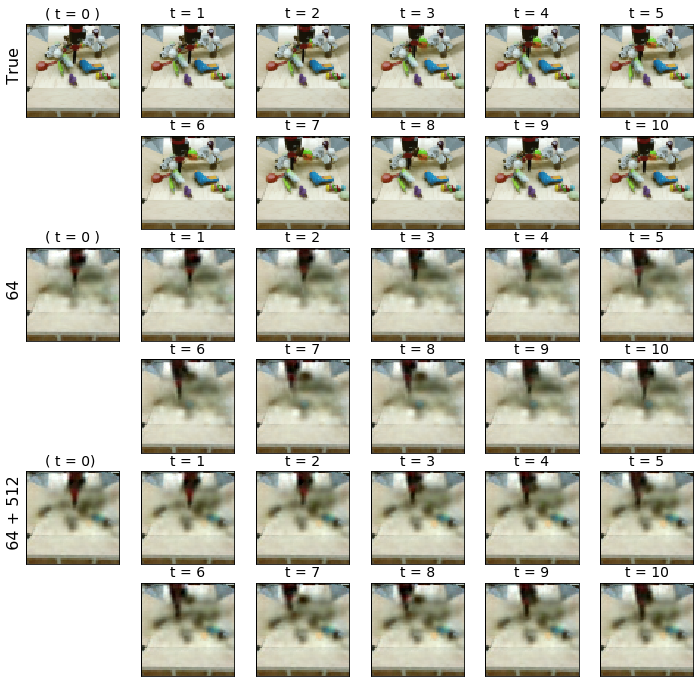
\includegraphics[width=0.75\linewidth]{./figures/pred_a.png}
      \caption[映像予測結果の比較]{\small 映像予測結果の比較.「True」が正解映像,「64」がベースライン(64)での予測結果,「64 + 512」が提案手法(64 + 512)での予測結果を示す.また$t = 0$は初期状態の推論時に与えられるフレームを示す.}
      \label{fig:pred_a}
  \end{center}
  \end{figure}
\normalsize

\section{考察}
生成結果がぼやけている点については画像のエンコードモデル・デコードモデルを大きくするなどの工夫で改善が見込めるが,物体の移動の予測が不十分な点は,DSSMが将来の観測の生成を通して状態表現を学習しているために,生成誤差にそれほど影響の出にくい小さい物体などは状態表現として獲得することがそもそも難しいことも原因だと考えられ,改善は難しいと思われる.また,画像を生成しやすい表現と遷移を考えやすい表現は必ずしも一致しないため,生成に依らない状態表現の学習手法も模索するべきであると考える.

\section{結論}

本研究では実機ロボットへの応用を見据えて深層状態空間モデルを用いた映像予測について取り上げ,提案手法によって映像予測の性能の改善を行った.深層状態空間モデルで映像予測を行う際の課題が多く発見できたので,今後の研究につなげていきたい.

\bibliography{references}
\bibliographystyle{unsrt}
%%%%%%%%%%%%%%%%%%%%%%%%%%%%%%%%%%%%%%%%%%%%%%%%%%
\end{document}